%! Author = adnansiddiquei
%! Date = 08/03/2024

\section{Experimentation, Profiling and Optimisation}\label{sec:profiling}
    This section discusses the experimentation and profiling of the different methods discussed in the previous
    section (Section \eqref{sec:prototyping}).
    Most of the experimentation was done on a Macbook M1 Pro (see Appendix \eqref{app:macbook-specs}), which is why the number of OpenMP threads for local
    experimentation was limited to 10.
    \subsection{Profiling the Convolution Methods}\label{subsec:prof-conv}
    \begin{figure}[htb]
    \centering
    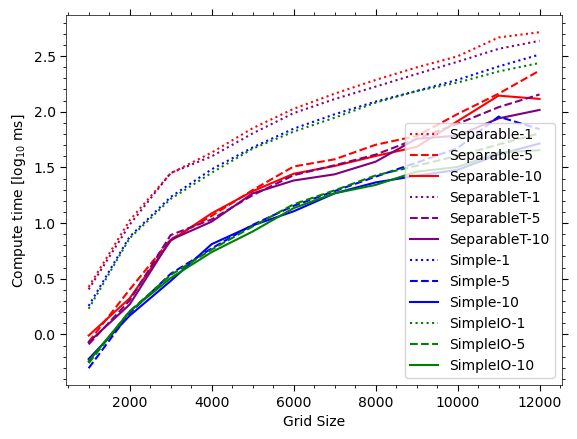
\includegraphics[width=0.75\textwidth]{./figures/convolutions}
    \caption{A figure showing the compute time for 4 of the convolution methods for counting neighbours.
        The colour of the line indicates the method used, and the line style (dotted, dashed, solid) indicates the number
        OpenMP threads used (1, 5 and 10 respectively).
        Only 1 MPI rank was used.
        The x-axis shows the size of one dimension of the square grid.
        The Simple and Separable methods are as described in \eqref{subsec:domain-decomp} and the SimpleIO method is
        as described in \eqref{subsec:hiding-comms})
        The SeparableT method is the Separable method done in 2 horizontal passes with a transpose in between, except
        the time on the graph is just the compute time to repeast the first horizontal pass twice (i.e, it is the time
        for the actual SeparableT method minus the tranpose compute time).
        This was done for simplicity, to assess whether a tranpose operation needed coding.
        The compute time is averaged over 3 runs.}
    \label{fig:convolutions}
    \end{figure}

    Fig.\eqref{fig:convolutions} shows the compute time across 4 different convolution methods for counting neighbours
    and how they scale with \inlinecode{grid_size} and \inlinecode{OMP_NUM_THREADS}.
    The first observation is that both the simple methods are faster than both of the separable methods, which is
    at face value, unexpected.
    Furthermore, there is a negligible difference in speed between the Simple and SimpleIO method which is a positive
    outcome which means the SimpleIO method is a good candidate for hiding communication overheads, as the vast majority
    of the computation can be done while waiting for the communication to complete.
    It is worth noting that all of these methods show diminishing returns as the number of OMP threads increases.

    It is worth noting that loop unrolling was implemented in all of these convolutions, the kernel was applied
    to the grid manually rather than having an additional loop (0 to 9) which applied the kernel.
    Whilst this was extra lines of code, experimentally, this was found to yield about a 2.5x speedup.
    Additionally, all of these double nested loops (which looped over the rows and columns of the grids) were parallelised
    using the OMP \inlinecode{parallel for collapse} clause which allowed OMP to collapse and parallelise the
    nested loops.

    \begin{figure}[htb]
    \centering
    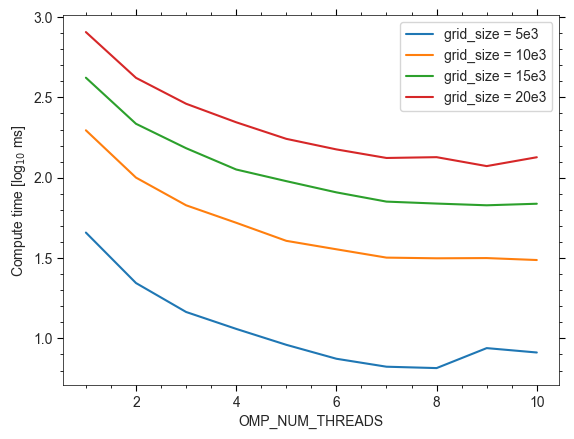
\includegraphics[width=0.75\textwidth]{./figures/simpleio}
    \caption{A figure showing how the compute time varies for the SimpleIO method as the number of OMP threads is changed.
    1 MPI rank was used, and compute time is averaged over 3 runs.}
    \label{fig:simpleio}
    \end{figure}

    Fig.\eqref{fig:simpleio} shows that as the number of OMP threads increases, the compute time decreases, but with
    diminishing returns.
    The jump from 1 to 2 threads yields a 2x increase but jumps following this do not yield speed increases in the same
    proportion.
    At about 8 threads, the returns on increasing the number of threads become negligible, which is useful information
    for optimising the MPI rank to OMP thread ratio.

    The analysis thus far has yielded the following conclusions: the SimpleIO method is a good candidate for counting
    neighbours and hiding MPI communication overheads; and 8 may be a reasonable cap on the optimal number of OMP threads
    (at least, for the M1 Pro chip).

    \subsection{Profiling the Update Methods}\label{subsec:prof-trans}
    \begin{figure}[htb]
    \centering
    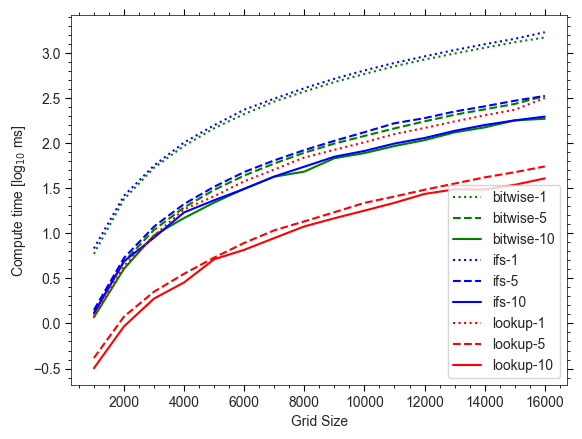
\includegraphics[width=0.75\textwidth]{./figures/transitions}
    \caption{A figure showing the compute time for the 3 the update methods discussed in Section \eqref{subsec:update-grid}.
        The colour of the line indicates the method used, and the line style (dotted, dashed, solid) indicates the number
        OpenMP threads used (1, 5 and 10 respectively).
        Only 1 MPI rank was used.
        The compute time is averaged over 3 runs.}
    \label{fig:transitions}
    \end{figure}

    Fig.\eqref{fig:transitions} explores the update methods discussed in Section \eqref{subsec:update-grid}, with a
    clear conclusion that the lookup method is the fastest, and as expected, the \inlinecode{if} method is the slowest.
    This makes sense, due to the (effectively) random nature of the simulation, the CPU will have little success
    in branch predictions, contributing to the slowness of the \inlinecode{if} method down.
    The frequent lookup in an 18-length array is relatively inexpensive compared to frequent branching.

    \begin{figure}[htb]
    \centering
    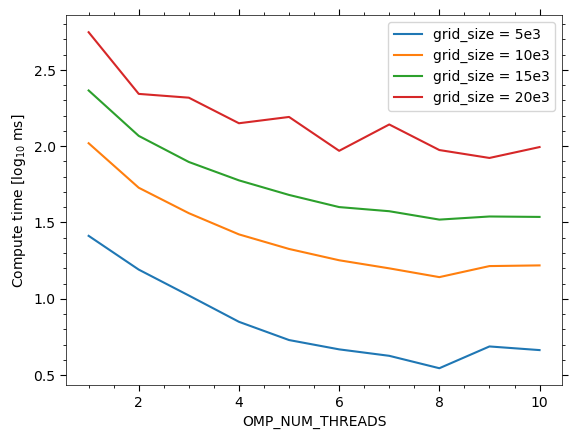
\includegraphics[width=0.75\textwidth]{./figures/lookup}
    \caption{A figure showing how the compute time varies for the updating the grid using the lookup method as the number
        of OMP threads is changed.
        1 MPI rank was used, and compute time is averaged over 5 runs.}
    \label{fig:lookup}
    \end{figure}

    Similar to Fig.\eqref{fig:simpleio}, Fig.\eqref{fig:lookup} shows that the lookup method for updating the grid starts
    to show diminishing returns in performance after about 8 OMP threads have been created.

    \subsection{Algorithm Conclusions}\label{subsec:interim-conclusions}
\begin{figure}[htb]
    \centering
    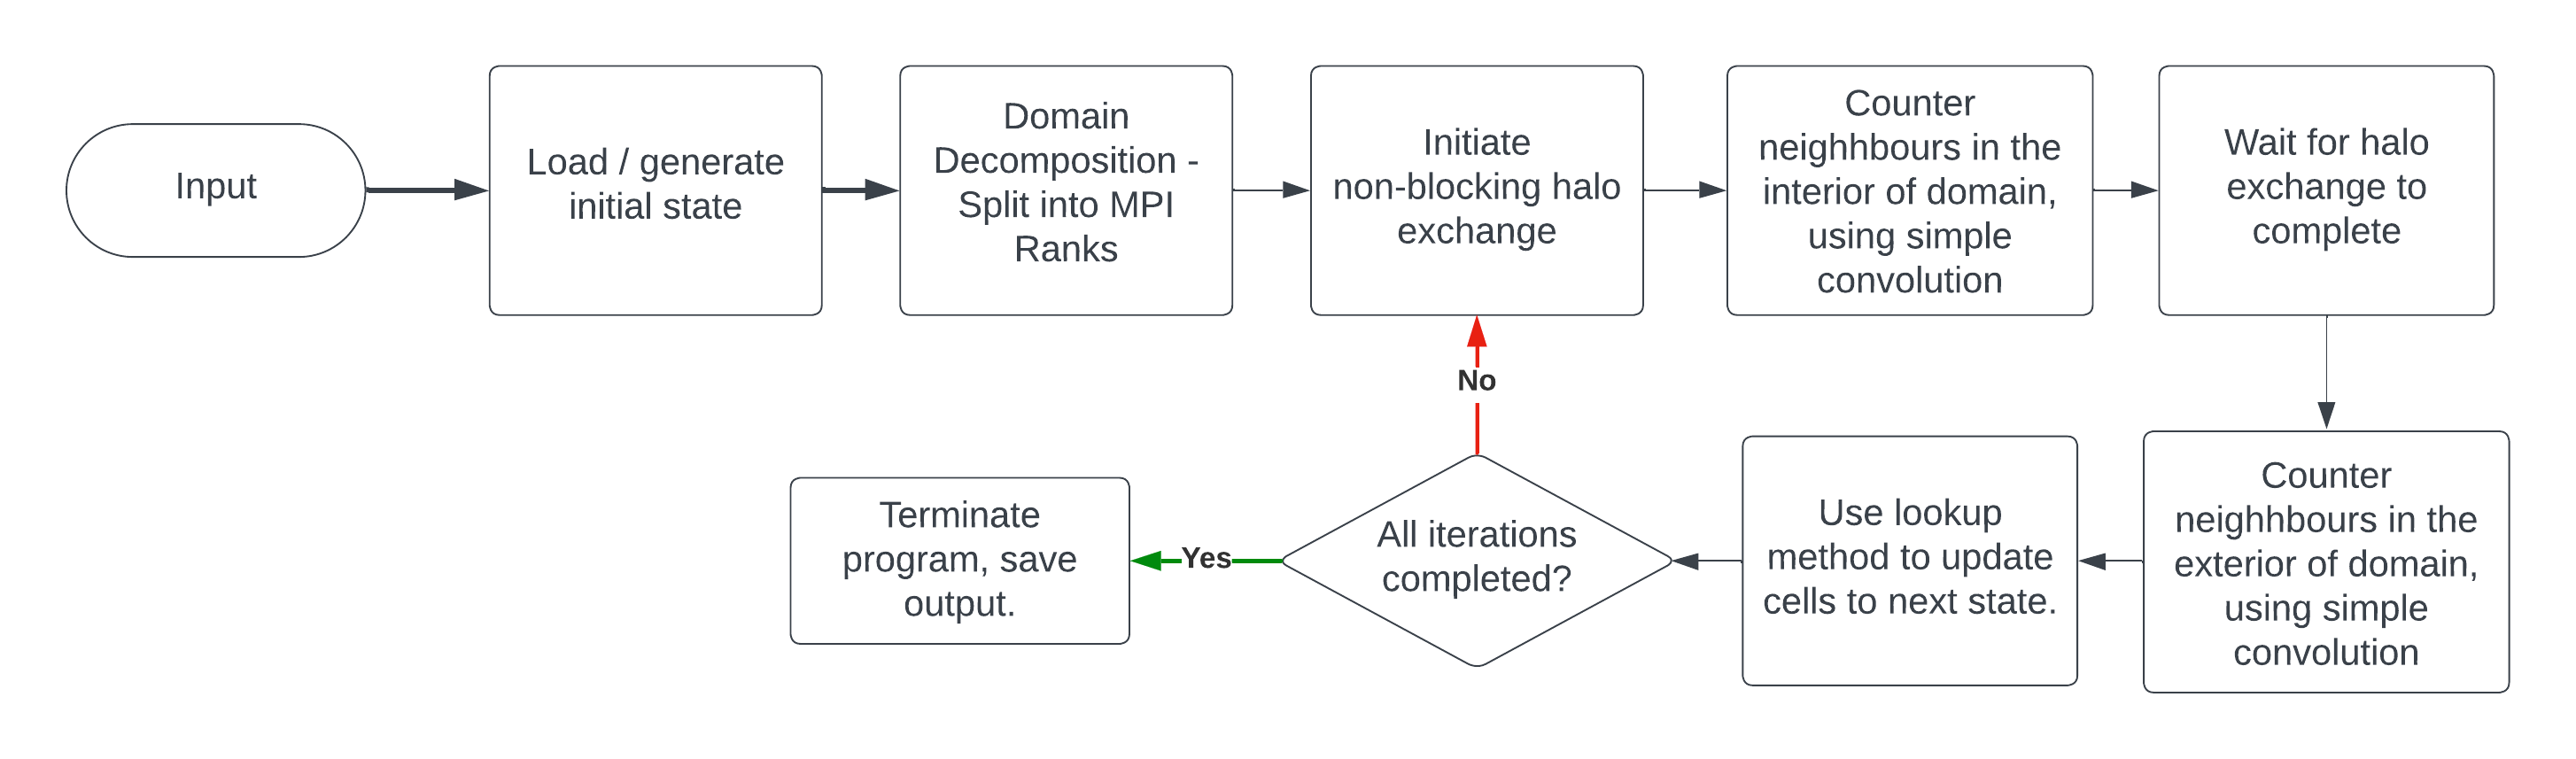
\includegraphics[width=0.75\textwidth]{./figures/flowchat-2}
    \caption{An updated version of Fig.\eqref{fig:high-level-flowchart} with the conclusions from the experimentation
    and profiling.}
    \label{fig:flowhcart-2}
    \end{figure}
    Given the performance testing of the neighbour counting and grid updating methods, the SimpleIO and lookup methods
    are the best candidates for the simulation.
    The SimpleIO can be used to hide communication overheads effectively and the lookup method is the fastest way to
    update the grid, Fig \eqref{fig:flowhcart-2} shows an updated flowchart of the overall algorithm.
    These conclusions are likely transferable to other architectures, but the exact number of OMP threads that yield
    the best performance will need to be re-evaluated for each architecture.
    It is likely that for the M1 Pro, the bottleneck at roughly 8 OMP threads is due to memory constraints rather
    than the algorithm itself not parallelising well, given that the datasets used in the simulation are large enough
    to completely fill L1 and shared L2 caches.

    The optimal domain decomposition was not explored due to time constraints, row-wise decomposition was implemented
    for the sake of simplicity and it was preferred over column-wise decomposition to reduce non-contiguous data
    exchange between MPI ranks.
    The last thing to explore is the optimal number of MPI ranks to use, and the optimal ratio of MPI ranks to OMP threads.

    \subsection{MPI Ranks and OMP Threads}\label{subsec:mpi-omp}
    The conclusions drawn in this section would be very system dependent, the results on an M1 Pro chip are unlikely
    to directly transfer to a HPC cluster.




